% !TEX root = ../../../main.tex
% 来源：中学数学实验教材·第二册（几何）
% 章节：集合与简易逻辑 / 简易逻辑
% 原始文件：2.tex，行 1176-1182
% 类型：tikz
% ---
    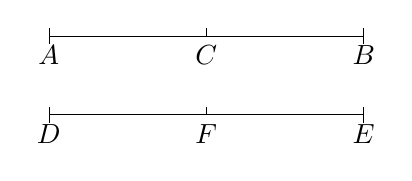
\begin{tikzpicture}[>=latex, scale=1]
      \draw[|-|](0,0)node[below]{$A$}--(4,0)node[below]{$B$};
\draw[|-|](0,-1)node[below]{$D$}--(4,-1)node[below]{$E$};
\node at (2,0)[below]{$C$};
\node at (2,-1)[below]{$F$};
\draw(2,0)--(2,.1);\draw(2,-1)--(2,-1+.1);
    \end{tikzpicture}
